\section{Day 23: No Retraction, Brouwer Fixed Point Theorem. Stone-Cech Compactification, Rigorous Definition of Limit (Nov. 26, 2024)}
Outfit of the day: monocolor sweater. that's a second
\begin{figure}[h]
    \centering
    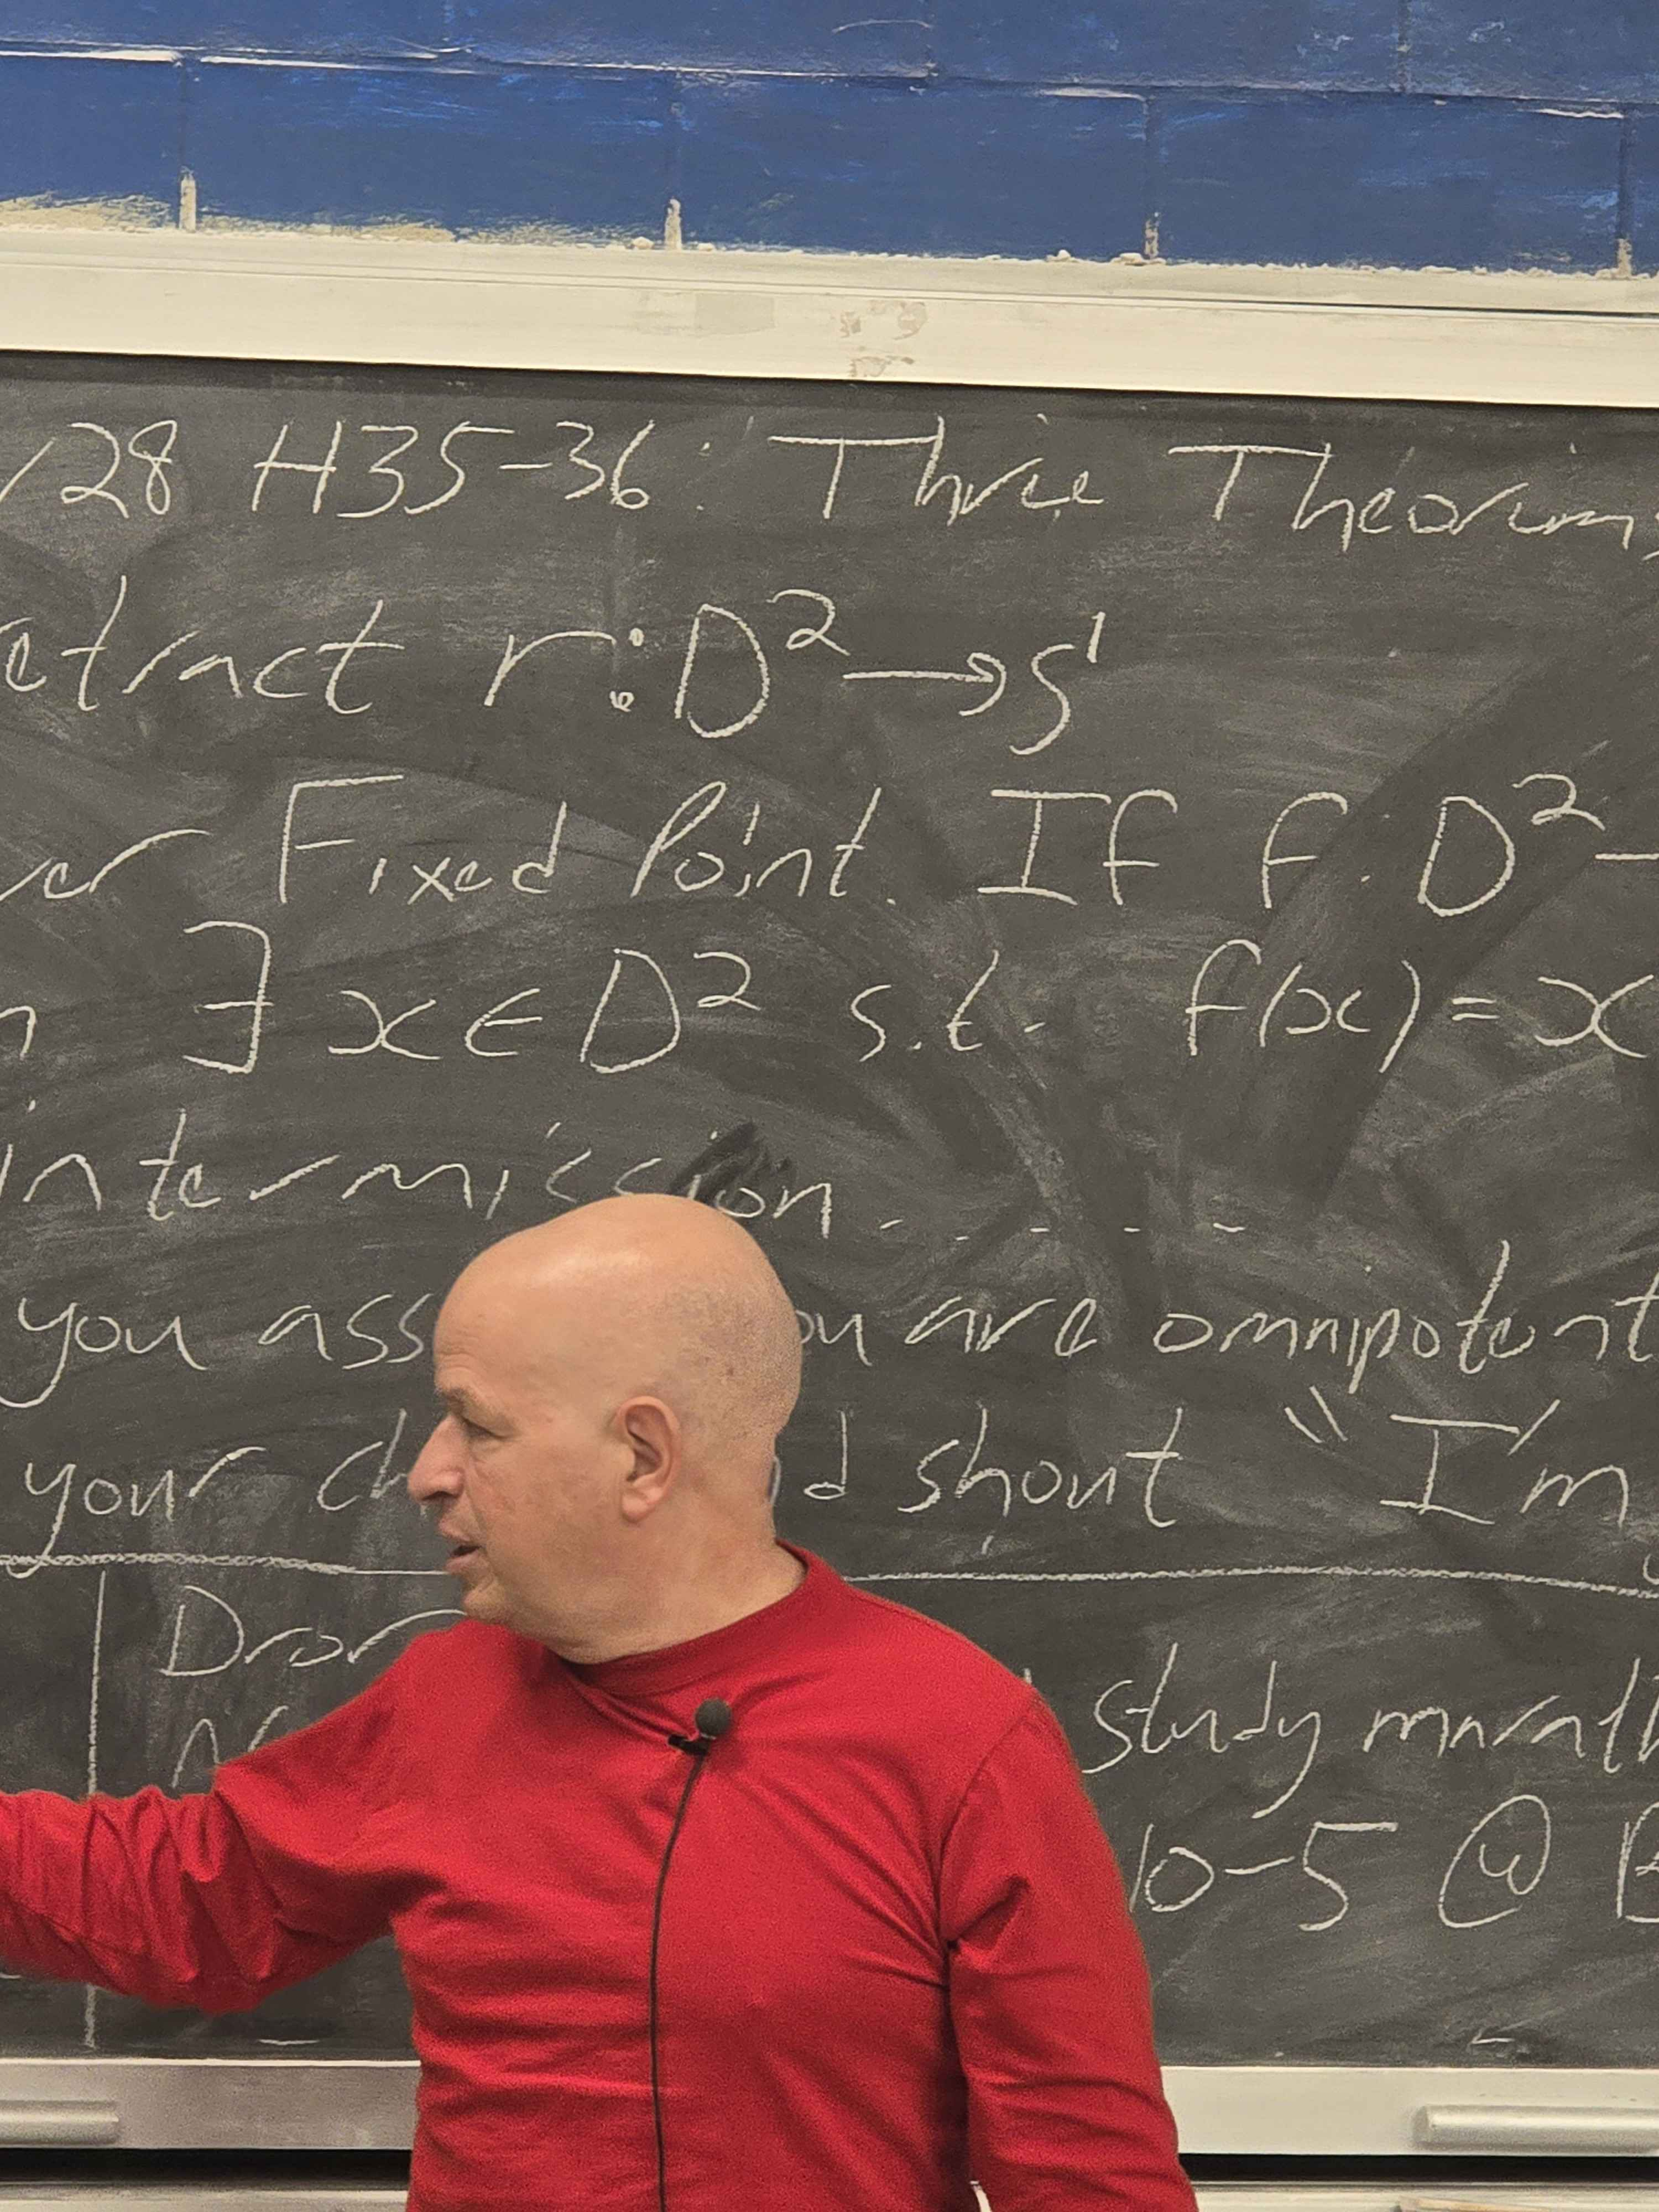
\includegraphics[scale=0.1]{MAT327 Notes/Dror Shirts/dror day 24 shirt.jpg}
\end{figure}

\noindent \textbf{Office hours information!}
\begin{itemize}
    \item Brinda will host office hours on Friday on Dec. 13, from 10am to 1pm in the grad lounge.
    \item Dror will not host office hours on Dec. 3, but will host them on Dec. 10, and will be available for a ``study marathon'' on Sunday, Dec. 15, from 10am to 5pm on Bahen's 6th Floor. He will roam around looking for topology students.
\end{itemize}

We will prove three major theorems today.
\begin{enumerate}[label=(\roman*)]
    \item There does not exist a retract $r : D^2 \to S^1$.
    \item (Brouwer Fixed Point Theorem) If $f : D^2 \to D^2$ is continuous, then there exists $x \in D^2$ such that $f(x) = x$.
    \item If you assume you are omnipotent, you get the pound on your chest and shout ``I'm great!''
\end{enumerate}
Recall that we have the following tools for today's lecture:
\[ \pi_1(\RR) = 0; \hspace{0.2in} \pi_1(S^1) = \ZZ, \]
and that $\pi_1$ is a functor, i.e.
\[
    \begin{tikzcd}
        X \arrow[r, rightsquigarrow, "\pi_1"] \arrow[loop left, "\id_X"] \arrow[d, "F"'] & \pi_1(X) \arrow[d, "\pi_1 f = f_\ast"] \\
        Y \arrow[r, rightsquigarrow, "\pi_1"'] \arrow[loop left, "\id_Y"] & \pi_2(Y)
    \end{tikzcd}
\]
We now prove the aforementioned theorems.
\begin{simplethm}[No Retraction]
    There does not exist a retract $r : D^2 \to S^1$.
\end{simplethm}
\noindent Suppose $r$ exists. Then we have the following diagram,
\[
    \begin{tikzcd}
        S^1 \arrow[r, hookrightarrow, "\iota"] \arrow[rd, "I"']& D^2 \arrow[d, "r"{name=L}] & \ZZ \arrow[r, "\pi_1 \iota"] \arrow[rd, "I"'{name=R}] & \{e\} \arrow[d, "\pi_1 r"] \\
        & S^1 & & \ZZ \arrow[from=L, to=R, start anchor = {[xshift=1ex]}, end anchor = {[xshift=-2ex, yshift=1.3ex]}, rightsquigarrow, "\pi_1"]
    \end{tikzcd}
\]
More generally, there does not exist a retraction $D^n \to S^{n-1}$ for $n > 2$, but this result will not be tested on the final. The proof is identical as the above, except we need a different functor.

\begin{simplethm}[Brouwer Fixed Point]
    If $f : D^2 \to D^2$ is continuous, then there exists $x \in D^2$ such that $f(x) = x$.
\end{simplethm}
\noindent By contradiction, assume $f : D^2 \to D^2$ is continuous and fro all $x$, $f(x) \neq x$. Let $r(x)$ be the point where the straight ray from $f(x)$ to $x$ is continuous, and hits the circle. Then $r(x)$ is continuous; if $x \in S^1$, then $r(x) = x$. So $r : D^2 \to S^1$ is a retract, but retracts don't exist. \qed
\medskip\newline
\noindent \textit{Everything from this point onwards is not going to be tested on the final.}

\begin{simplethm}[Formality of Limit]
    Assuming the axiom of choice, then let $\mathrm{Lim}$ be a function be from bounded sequences to $\RR$ such that
    \begin{enumerate}[label=(\roman*)]
        \item $\mathrm{Lim}$ is linear, i.e. $\mathrm{Lim}(a_n + b_n) = \mathrm{Lim} \, a_n + \mathrm{Lim} \, b_n$, and $\mathrm{Lim} \, (ca_n) = c \mathrm{Lim} \, a_n$, 
        \item $\mathrm{Lim} (a_n b_n) = (\mathrm{Lim} \, a_n)(\mathrm{Lim} \, b_n)$
        \item $\mathrm{Lim} \, a \in \bigcap_n \overline{\{a_k \mid k \geq n\}}$. If $a$ is convergent, then $\mathrm{Lim} \, a = \lim a$.
    \end{enumerate}
\end{simplethm}
\noindent Note that $\limsup$ doesn't really possess any ``nice'' linearity properties. We also cannot ask that $\mathrm{Lim}$ have the property
\begin{enumerate}[label=(\roman*)]
    \setcounter{enumi}{3}
    \item $\mathrm{Lim} \, a_{n+1} = \mathrm{Lim} \, a_n$, since we can just take the sequences $a_n = 0$ if $n$ is odd, and $1$ if even.
\end{enumerate}
Reminder that the axiom of choice implies Tychonoff's theorem; if $X_\alpha$ is compact, then for all $\alpha$, we have that $\prod_{\alpha} X_\alpha$ is compact. We instead assume the version that $I^W$ is compact even if $W$ is huge.
\medskip\newline
We now prove (iii). Let $W$ be the set of all bounded real sequences. For $a \in W$, let $I_a = [\inf a, \sup a] \ni a_k$. Let $X = \prod_{a \in W} I_a$, which is compact. Let $\alpha : \NN \to X$ be given by $\alpha(n)_a = a_n$. Then $\alpha$ is an embedding, meaning that $\alpha$ is a homeomorphism into its image. This means that it is continuous, $\alpha$ is injective, and that $\alpha(\NN)$ is discrete.
\medskip\newline
\noindent Continuity is automatically given; the second property is given by observing that if $n \neq m$, then we may pick $a$ such that $a_n \neq a_m$, and then we have $\alpha(n)_a = a_n \neq a_m = \alpha(m)_a$. Given $n$, let $a_k^n = \delta_{nk}$, where $\delta$ is the Kronecker delta. Then $a^n = (0, \dots, 0, 1, 0, \dots, 0)$. Let $U_n = \prod_{a^n}^{-1} \left(\frac{1}{2}, \frac{3}{2}\right)$. Then $\alpha(m) \in U_n$ if and only if $\pi_{a^n}(\alpha(m)) \in \left(\frac{1}{2}, \frac{3}{2}\right)$, i.e. $a_m^n \in \left(\frac{1}{2}, \frac{3}{2}\right)$, which is true if and only if $m = n$ by the Kronecker delta.
\medskip\newline
Now, let $\beta \NN = \overline{\alpha(\NN)}$, i.e. the ``Stone-Cech compactification of $\NN$'' Clearly, this is compact, so $\alpha(\NN) \neq \beta \NN$ (more specifically, the former is included, but not equal to).

\begin{simpleclaim}
    Every bounded sequence $a$ extends uniquely to a continuous $\tilde{a} : \beta \NN \to \RR$.
\end{simpleclaim}
\noindent Note that the diagram is given by
\[
    \begin{tikzcd}
        \NN \arrow[rr, "\alpha"] \arrow[dr, "a"'] & & \beta \NN \arrow[dl, "\tilde{a}"] \\
        & \RR &
    \end{tikzcd}
\]
Given $a$ and $\mu \in \beta \NN$, set $\tilde{a}(\mu) = \mu_a$, i.e. $\tilde{a} = \restr{\pi_a}{\beta \NN}$. It is continuous, and $\tilde{\alpha}(\alpha(n)) = \alpha(n)_a = a_n$. It is also unique since, for $b, c : \beta \NN \to \RR$ such that 
\[
    \begin{tikzcd}
        \NN \arrow[rr, "\alpha"] \arrow[dr, "a"'] & & \beta \NN \arrow[dl, "b"] \arrow[dl, "c"', shift right = 1ex] \\
        & \RR &
    \end{tikzcd}
\]
then $\restr{b}{\Ima \alpha} = \restr{c}{\Ima \alpha}$, but $\Ima \alpha$ is dense in $\beta \NN$, so by the term test, we must have $b = c$. Now, pick any point $\mu \in \beta \NN \setminus \alpha(\NN)$, which exists because of axiom of choice.  Define $\mathrm{Lim} \, a = \mathrm{Lim}_\mu a = \tilde{a}(\mu) = \mu_a = \pi_a (\mu)$.
\begin{simpleclaim}
    If $F : \RR^2 \to \RR$, then $\mathrm{Lim} \, F(a_n, b_n) = F(\mathrm{Lim} \, a_n, \mathrm{Lim} \, b_n)$.
\end{simpleclaim}
\noindent Let $F(\tilde{a}, \tilde{b})$, $F(a, b)$ be functions $\beta \NN \times \beta \NN \to \RR \times \RR \to \RR$, where the composition is given by $\tilde{a} \circ F$, $\tilde{b} \circ F$ respectively. Note that $F(\tilde{a}, \tilde{b}) = \widetilde{F(a, b)}$ since the extension of $F(a, b)$ to $\beta \NN$ is unique. Evaluating on $\mu$, we get
\[ F(\mathrm{Lim} \, a, \mathrm{Lim} \, b) = F(\tilde{a}(\mu), \tilde{b}(\mu)) = \mathrm{Lim} \, F(a, b). \qed \]

\begin{simpleclaim}
    For all $n$, $\mathrm{Lim} \, a \in \overline{\{ a_k \mid g \geq n \}}$.
\end{simpleclaim}
\noindent Let $\mu \in \overline{\alpha (\NN_{\geq n})}$. Let $\mu \in \overline{\alpha(\NN)} = \alpha(\NN)$, so $\mu \in \alpha(\NN)'$. So every neighborhood of $\mu$ contains infinitely many of the $\alpha(\NN)$'s as desired. Applying $\pi_a$, we have that
\[ \mathrm{Lim} \, a = \pi_a(\mu) \in \pi_a( \overline{\alpha (\NN_{\geq n})} ) \subset \overline{\pi_a \left(\alpha (\NN_{\geq n}) \right)}. \]
This is the first time we're using that if $f$ is continuous, then $f(\overline{A}) \subset \overline{f(A)}$. In particular, we have
\[ \overline{\pi_a \left(\alpha (\NN_{\geq n}) \right)} = \overline{\{\pi_a (\alpha(k)) \mid k \geq n\}} = \overline{\{\alpha(k)_a \mid k \geq n\}} = \overline{\{a_k \mid k \geq n\}}. \qed \]